\subsubsection{Errori possibili}\label{errori-possibili}

Con la formulazione delle due ipotesi è possibile commettere due tipi di
errori:

\begin{itemize}
\item
  \textbf{errore di primo tipo}: viene rifiutata $ H_0 $ quando questa è
  vera.
\item
  \textbf{errore di secondo tipo}: accettare $ H_0 $ quando $ H_0 $ è falsa.
\end{itemize}

Per come è stato costruito il test statistico si ha che

$$
P(\text{errore 1° tipo}) = 1 - P(\text{accettare } H_0 \text{ quando è vera})
$$

e viene fissato ad $\alpha$, perché

$$ P(\text{accettare } H_0 \text{ quando è vera}) = 1- \alpha $$

Tuttavia non viene detto nulla a riguardo dell'errore del secondo tipo.
Si sa solo che non si possono minimizzare i due errori
contemporaneamente, perché sono tra loro correlati.

Ma alla fine quello che conta è l'errore di primo tipo, perché la
domanda che ci si pone è ``\emph{A:i dati sperimentali sono compatibili
con $ H_0 $?}'' piuttosto che ``\emph{B:Quale tra $ H_0 $ e $ H_1 $ è vera?}''.

L'approccio adottato prevede quindi di fissare l'errore più importante
(con $\alpha$) e minimizzare la probabilità d'errore del secondo
tipo.

Sfruttando i dati è comunque possibile ridurre entrambi i tipi d'errore
perché se il numero \emph{n} di dati a disposizione è grande e quanto
più è dispersa la variabile esplicativa, tanto più gli errori commessi
sono minori.

\subsection{Rilassando le ipotesi}\label{commenti}

Finora è stato assunto che i dati seguano una distribuzione normale,
quindi prima di effettuare una regressione lineare è necessario andare a
verificare che questo sia vero.

Per effettuare questa verifica servono delle tecniche grafiche ed
analitiche complesse, pertanto è più ragionevole utilizzare un approccio
alternativo che verifica a posteriori la normalità dei dati.

Un'altra ipotesi fatta riguarda la conoscenza della varianze delle
distribuzione, ma nel lato pratico questo è un parametro ignoto.

Utilizzando il metodo dei minimi quadrati è possibile solamente stimare
i coefficienti beta e non la varianza.

Tuttavia, considerando $y = \beta_0 + \beta_1x + \epsilon$, si può
isolare $\epsilon$ e stimarlo utilizzando i residui osservati:

\begin{align*}
	\hat{\epsilon}_i ) &= r_i = y_i - \hat{y}_i = \\
								  &= y_i - \hat{\beta}_0 - \hat{\beta}_1x_i
\end{align*}


Si può quindi costruire uno stimatore per la varianza della componente di
errore utilizzando la varianza dei residui\footnote{La media dei residui è 0.} che è facilmente calcolabile.

\begin{align*} 
	\hat{\sigma}^2 &= \frac{1}{n}\sum\limits_{i=1}^n (r_{i} - 0)^2\\
								&= \frac{1}{n}\sum\limits_{i=1}^n (y_i - \hat{\beta}_0 - \hat{\beta}_1x_i)^2
\end{align*}

Utilizzando questo stimatore si tende ad ottenere \textbf{una sottostima} della varianza, pertanto conviene utilizzare

\begin{align*} 
\hat{s}^2 &= \frac{1}{n-2}\sum\limits_{i=1}^n (r_{i} - 0)^2\\
				 &= \frac{1}{n-2}\sum\limits_{i=1}^n (y_i - \hat{\beta}_0 - \hat{\beta}_1x_i)^2
\end{align*}

\subsubsection{Il problema di verifica delle ipotesi senza $\sigma^2$}\label{il-problema-di-verifica-delle-ipotesi-senza-sigma2}

Dal momento che non è nota la varianza, non è più possibile utilizzare $ z $ per effettuare la verifica dell'ipotesi su $ \beta_1 $, ma è necessario utilizzare un'altra statistica test:

$$
t_{oss} = \frac{(\hat{\beta}_1 - 0)}{\sqrt{\frac{s^2}{\sum_{i=1}^{n} (x_i - \bar{x})^2}}}
$$

Il pedice \textit{oss} indica che viene influenzata dai dati osservati.

Il funzionamento di $ t_{oss} $ è analogo a quello di $ z $: se $ H_0 $ è vera, ci si aspetta che $ t_{oss} $ assuma valori vicini allo 0.

Per determinare il valore di $ t_{oss} $ non è possibile utilizzare la distribuzione normale, perché la varianza non è nota, ed è quindi necessario utilizzare la \textbf{\textit{t} di Student}\footnote{Questo è possibile perché nelle nostre ipotesi gli errori seguono la distribuzione normale e sono tra loro indipendenti.}.

La distribuzione \emph{t di Student} dipende da un solo parametro che
prende il nome di \textbf{gradi di libertà}. Durante a verifica
dell'ipotesi sul coefficiente angolare della retta di regressione, il
grado di libertà è \emph{n-2}, ovvero è stato dimostrato che:

$$
t_{oss} \approx t \text{ di Student con } n - 2 \text{ gradi di libertà.}
$$

Il grafico di questa distribuzione è simile a quello della normale, solo
che ha delle code più pesanti.

\begin{figure}[htbp]
\centering
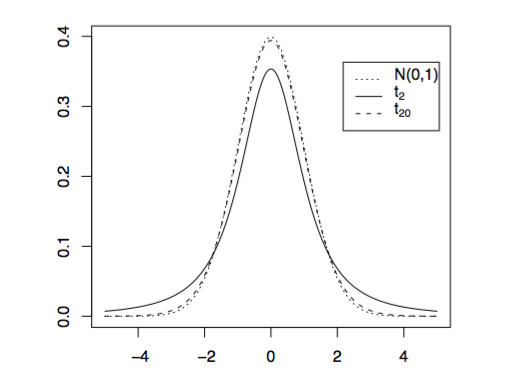
\includegraphics{./notes/immagini/l6-fig5.png}
\caption{Confronto della $ t $ di Student con la normale $ \mathcal{N}(0,1) $}
\end{figure}

In questo caso però non conviene utilizzare un confronto sulla soglia dei valori, perché questo potrebbe enfatizzare troppo delle differenze minime, portando a dei valori completamente diversi.

L'idea è quindi quello di fissare un \textbf{livello di significatività
osservato} o \textbf{p-value} uguale alla probabilità di osservare sotto
$ H_0 $ un valore di $ t_{oss} $ più o ugualmente lontano da $ H_0 $ di quanto
effettivamente è osservato.

\begin{figure}[htbp]
\centering
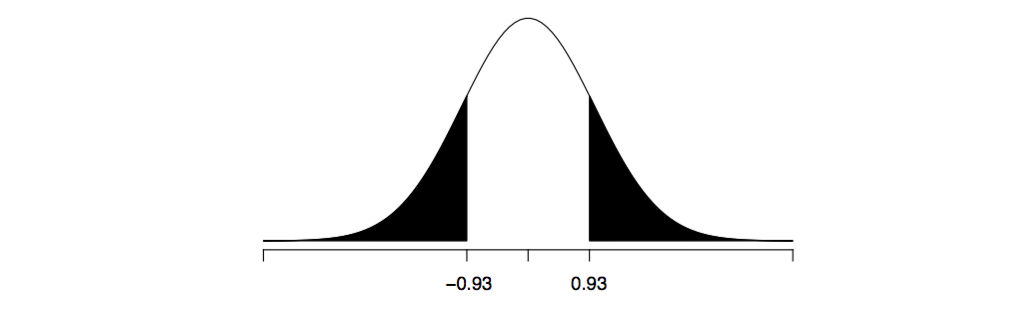
\includegraphics{./notes/immagini/l6-fig7.png}
\caption{La curva mostra la densità di una t di Student. Poiché lontano da 0 vuol dire lontano da $ H_0 $, l'area annerita fornisce una approssimazione della probabilità di osservare, quando è vera $ H_0 $, un valore più lontano dall'ipotesi nulla, rispetto a quanto osservato.}
\end{figure}

Il livello di significatività osservato costituisce una misura di quanto
l'ipotesi nulla è plausibile sulla base dei dati.

Questo livello varia da 0 a 1 e più è grande, più i dati sono vicini ad $ H_0 $.

\begin{itemize}
\item
  Se vale 0 vuol dire che sotto $ H_0 $ non è possibile osservare nessun
  altro valore più lontano da $ H_0 $, ovvero il valore osservato per $ t_{oss} $
  è uno dei più lontani possibili.
\item
  Se vale 1 vuol dire che sotto $ H_0 $ tutti i possibili valori osservabili
  per $ t_{oss} $ sono ``non più vicini di quello osservato, ovvero quello
  osservato è uno dei più vicini possibili.
\end{itemize}

\emph{lontano da $ H_0 $} equivale a dire \emph{``lontano da 0 in entrambe le
direzione''} quindi, nel caso delle vendite:

\begin{align*}
\text{livello di significatività osserato } &= P(|t \text{con 198 gradi}| \geq 9.921) \\
														           &= 2xP(t \text{con 198 gradi} \geq 9.921)
\end{align*}

Il calcolo della probabilità viene poi fatto utilizzando una tabella o
un software apposito. Nell'esempio si ha che il livello di significatività osservato è 0.

Ovvero, che se la spesa in pubblicità via radio ha un effetto sulle vendite allora noi ci aspetteremo valori ``Più lontani da $ H_0 $ di quanto
osservato''.

Il che vuol dire che il valore osservato di $ t_{oss} $ è molto strano (poco plausibile) quando $ H_0 $ è vera.

\paragraph{Interpretazione alternativa del $ p_value $} Supponendo di formare tutti i possibili campioni di 200 elementi e di calcolare $ t_{oss} $ per ognuno di questi. Allora il $ p-value $ è la percentuale di valori di $ t_{oss} $ maggiori di 9.921\footnote{Valore di $ t_{oss} $ calcolato per il data set d'esempio delle slide}, che per quanto calcolato prima ci si aspetta che sia 0. Ma allora 9.921 è un valore che difficilmente può capitare quando $ H_0 $ è vera, e quindi i dati smentiscono l'ipotesi nulla, che è da rifiutare.

\subsubsection{Intervallo di confidenza}\label{intevallo-di-confidenza}

\begin{figure}[htbp]
\centering
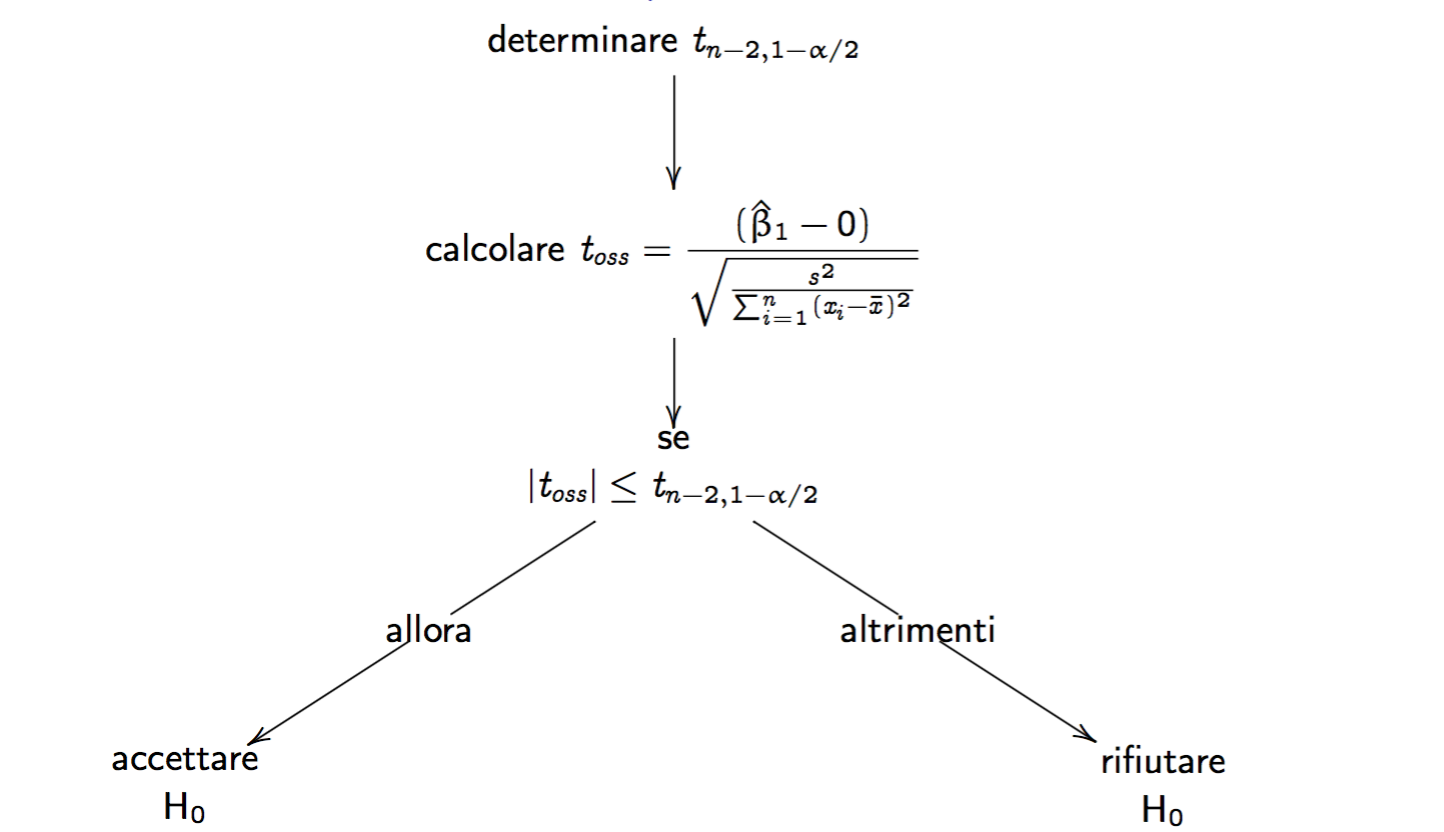
\includegraphics[width=.9\textwidth]{./notes/immagini/l6-fig9-1.png}
\caption{Regola per l'accettazione o il rifiuto di $ H_0 $. $ t_{g,p} $ indica il percentile $ p $-esimo di una \textit{t} di Student con \textit{g} gradi di libertà. L'albero fornisce una regola che garantisce di accettare $ H_0 $ quando questa è vera con probabilità $ 1 - \alpha $.}
\end{figure}

In modo analogo a come è stato fatto nel caso di $ \sigma^2 $ noto è possibile definire un'intervallo di confidenza per la stima.

$$
P\Bigg( -t_{n-2, 1-\alpha/2} \leq \frac{(\hat{\beta}_1 - \beta_1)}{\sqrt{\frac{s^2}{\sum_{i=i}^{n} (x_i - \bar{x})^2}}}\leq  t_{n-2, 1-\alpha/2}\Bigg) = 1 - \alpha
$$

Da cui si deriva che:

$$
\Bigg[ \hat{\beta}_1 -  \sqrt{\frac{s^2}{\sum_{i=i}^{n} (x_i - \bar{x})^2}} , \hat{\beta}_1 + \sqrt{\frac{s^2}{\sum_{i=i}^{n} (x_i - \bar{x})^2}}  \Bigg]
$$

\subsection{Verifica di ipotesi su $ \beta_0 $}\label{verifica-di-ipotesi-su-beta0}

In modo simile è possibile stimare $ \beta_0 $, anche se risulta molto meno
interessante, perché è $ \beta_1 $ che fornisce la relazione tra le \emph{x} e
le \emph{y}.

Come prima cosa è necessario stimare la varianza di $ \hat{\beta}_0 $:

$$
Var(\hat{\beta}_0) = \frac{\sum_{i=1}^{n} x_{i}^2}{n \sum_{i=1}^{n} (x_i - \bar{x})^2}s^2
$$

Le ipotesi diventano

$$
\begin{cases}
H_0 : \beta_0 = \beta' \\
H_1 : \beta_0 \neq \beta' 
\end{cases}
$$

dove $ \beta' $ è un valore fissato, ad esempio 0.

La statistica test diventa quindi:

$$
t_{oss}  = (\hat{\beta}_0 - \beta') \Bigg/ s \sqrt{\frac{\sum_{i=1}^{n} x_{i}^2}{n \sum_{i=1}^{n} (x_i - \bar{x})^2}}
$$

con intervallo di confidenza definito da

$$
\Bigg[ \hat{\beta}_0 - t_{n-2, 1-\alpha/2} s \sqrt{\frac{\sum_{i=1}^{n} x_{i}^2}{n \sum_{i=1}^{n} (x_i - \bar{x})^2}} \:,\: \hat{\beta}_0 + t_{n-2, 1-\alpha/2} s \sqrt{\frac{\sum_{i=1}^{n} x_{i}^2}{n \sum_{i=1}^{n} (x_i - \bar{x})^2}}\Bigg]
$$

Da notare che in questo modo non viene definito un intervallo di confidenza simultaneo, ovvero che vale sia per $ \beta_0 $ che per $ \beta_1 $.


\subsection{Verifica di ipotesi globale sul modello}\label{verifica-di-ipotesi-globale-sul-modello}

Per misurare la varianza spiegata dal modello abbiamo il coefficiente di
determinazione $R^2$ che misura la varianza spiegata dal modello
rispetto a quella complessiva. Non abbiamo però un criterio per capire
se l'$R^{2}$ osservato è grande o piccolo.

Anche in questo caso è possibile impostare un problema di verifica di
ipotesi, l'ipotesi nulla sarà l'indipendenza lineare tra \emph{x} e
\emph{y}, mentre l'ipotesi alternativa prevederà che la retta spieghi,
almeno in parte, la relazione presente.

Generalmente la statistica test più utilizzata per questo problema è:

$$
F_{oss} = \frac{\frac{R^2}{k -1}}{\frac{1-R^2}{n-k}} = \Bigg( \frac{R^2}{1-R^2} \Bigg) \Bigg( \frac{n-k}{k-1}\Bigg)
$$

dove \textit{k} rappresenta il numero di parametri utilizzati nel modello, nel nostro caso 2.

La statistica $ F_{oss}  $ può essere anche vista come il rapporto tra la media dei quadrati degli scarti spiegati dal modello e la corrispondente media dei quadrati degli scarti residui, pertanto ci aspettiamo $ F_{oss}  $ grande quando $ H_0 $ è falsa.

Nelle ipotesi di normalità ed indipendenza degli errori, si ha che $ F_{oss} $ si distribuisce come una variabile aleatoria detta \textbf{\textit{F} di Snedecor} con $ k-1 $ gradi di libertà al numeratore e $ n-k $ gradi di libertà al denominatore.

Il valore $ F_{oss} $ deve essere quindi confrontato con la \textit{F} di Snedecor utilizzando una tavola dei percentili o con un apposito software. Maggiore è $ F_{oss} $, minore è la probabilità che $ H_0 $ sia vera.

Ad esempio, con $ F_{oss}  = 98.42 $ si ha che il valore osservato è molto più grande del quantile $ 0.999 (\text{che vale circa } 11.15)$, sia ha quindi che la probabilità di osservare un valore uguale o più lontano da $ H_0 $ rispetto a quando osservato è inferiore di un millesimo.
I dati suggeriscono quindi che nel campione osservato si presenta una dipendenza lineare tra \textit{x} e \textit{y} e anche che questa dipendenza dovrebbe esserci in tutta la popolazione.

Il livello di significatività osservato fornisce quindi la probabilità di ottene una statistica \textit{F} maggiore o uguale a quella ottenuta dai dati a disposizione nel caso ci sia indipendenza tra \textit{x} e \textit{y}.

Il vantaggio di questo livello è che nasconde tutti i dettagli riguardo la statistica test.

Tipicamente, se il livello di significatività osservato è inferiore a $ 0.01 $ i risultati sono considerati altamente significativi \textbf{contro} $ H_0 $, mentre se risulta compreso tra $ 0.01 $ e $ 0.05 $ i risultati sono comunque significativi contro $ H_0 $, ovvero è molto probabile che $ H_0 $ sia falsa.

Viceversa, se risulta maggiore di $ 0.1 $ si conclude che i dati non contengono elementi tali da poter rifiutare $ H_0 $ e quindi sono \textbf{non significativi}.

\section{Effettuare previsioni}\label{effettuare-previsioni}

Una volta fatto il modello, è carino utilizzarlo per effettuare delle
previsioni o delle simulazioni sul futuro.

Questo può essere fatto fissando un determinato valore $ x0 $ e calcolando \textit{y} utilizzando i coefficienti stimati:

$$
\hat{y}_0 = \hat{\beta}_0 + \hat{\beta}_1 x_0
$$

Tuttavia può essere interessante avere anche un intervallo di precisione da associare alla stima $ \hat{y}_0 $.

Partendo dal modello di riferimento si ottiene:

\begin{align*}
	\hat{y}_0 &= \hat{\beta}_0 + \hat{\beta}_1 x_0 + \epsilon \\
					&= (\bar{y} - \hat{\beta}_1 \bar{x}) + \hat{\beta}_1 x_0 + \epsilon \\
					&= \bar{y} + \hat{\beta}_1(x_0 \bar{x}) + \epsilon 
\end{align*}

Si ha quindi che:

\begin{align*}
	Var(\hat{y}_0) &= Var(\bar{y}) + Var(\hat{\beta}_1)(x_0 - \hat{x})^2 + Var(\epsilon) \\
	                         &= \sigma^2 \Bigg( 1 + \frac{1}{n} + \frac{(x_0 - \hat{x})^2}{\sum_{i=1}^{n}} (x_i - \hat{x})^2 \Bigg)
\end{align*}

che può essere stimata utilizzando $ s^2 $ al posto di $ \sigma^2 $

$$
\widehat{Var(\hat{y}_0)} = s^2 \Bigg( 1 + \frac{1}{n} + \frac{(x_0 - \hat{x})^2}{\sum_{i=1}^{n}} (x_i - \hat{x})^2 \Bigg)
$$

L'intervallo di precisione risulta quindi essere

$$
\Bigg[ \hat{y}_0 - t_{n-2, 1-\alpha/2}\sqrt{\widehat{Var(\hat{y}_0)}} \:, \:\hat{y}_0 + t_{n-2, 1-\alpha/2}\sqrt{\widehat{Var(\hat{y}_0)}}\Bigg]
$$

Nell'esempio delle vendite, se $ x_0 = 60 $ si ottiene $ y_0 = 21.4614 $ con un intervallo di previsione $ [12.88 \; , \: 30.04] $ valido con il $ 95\% $ di probabilità.

Effettuando il calcolo dell'intervallo per ogni punto del dominio è possibile ottenere un grafico che rappresenta le \textbf{bande di previsione} ottenute.

\begin{figure}[htbp]
\centering
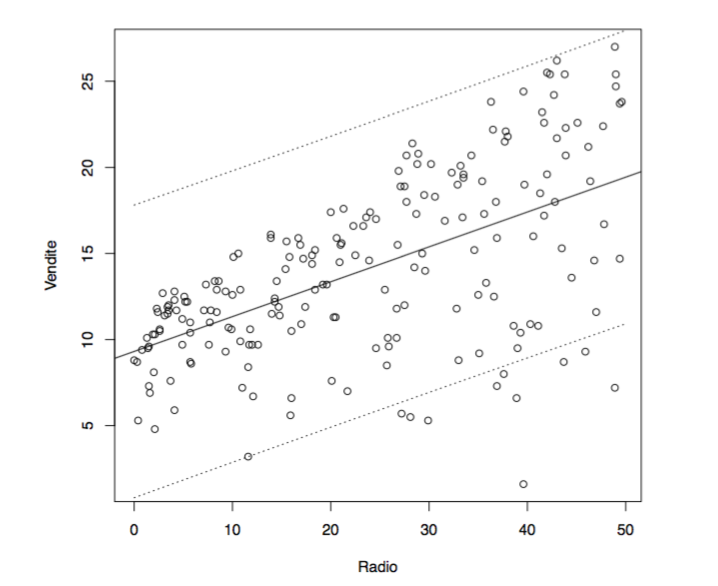
\includegraphics[width=.6\textwidth]{./notes/immagini/l6-fig10-1.png}
\caption{Bande di previsione}
\end{figure}

\subsection{Verifica del modello mediante i residui}

Anche le previsioni sono influenza dalle ipotesi riguardo la distribuzione degli errori e alla non variabilità della varianza.
Può succedere che i dati analizzati non soddisfino queste ipotesi ed è necessario avere degli strumenti che permettono di identificare questi casi.

Il modo più semplice per verificare ciò è rappresentare con un grafico, ad esempio con un istogramma, la distribuzione dei residui per osservare se questa ha la classica forma campanulare della distribuzione normale.

\begin{figure}[htbp]
\centering
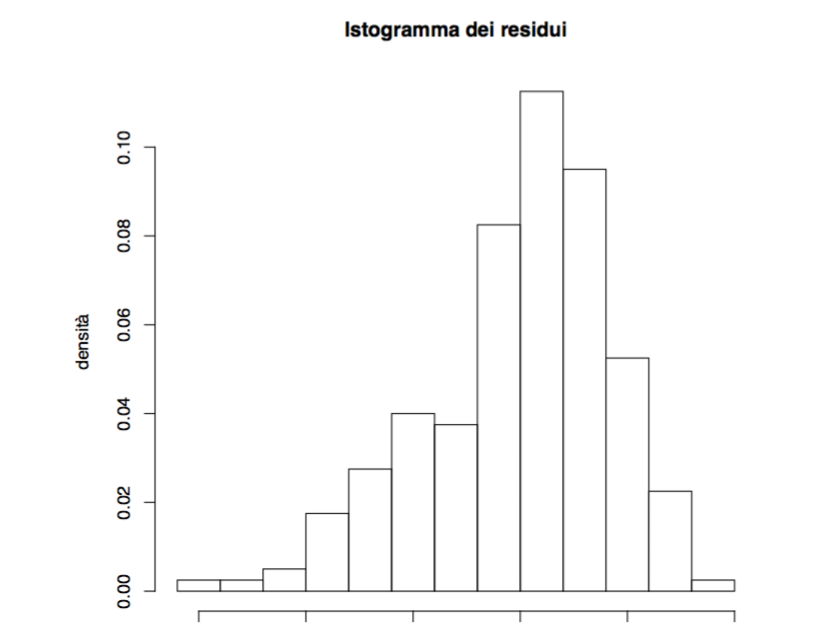
\includegraphics[width=.6\textwidth]{./notes/immagini/l6-fig11-1.png}
\caption{Istogramma dei residui per il data set delle vendite. In questo caso la campana non è proprio centrata, ma questo può essere dovuto a fattori casuali.}
\end{figure}

Un altro grafico che può è il tracciamento dei residui rispetto la stima $ \hat{y} $ ottenuta il quale aiuta a cogliere alcuni aspetti che ci aspettiamo vengano rappresentati dal modello.

\begin{figure}[htbp]
\centering
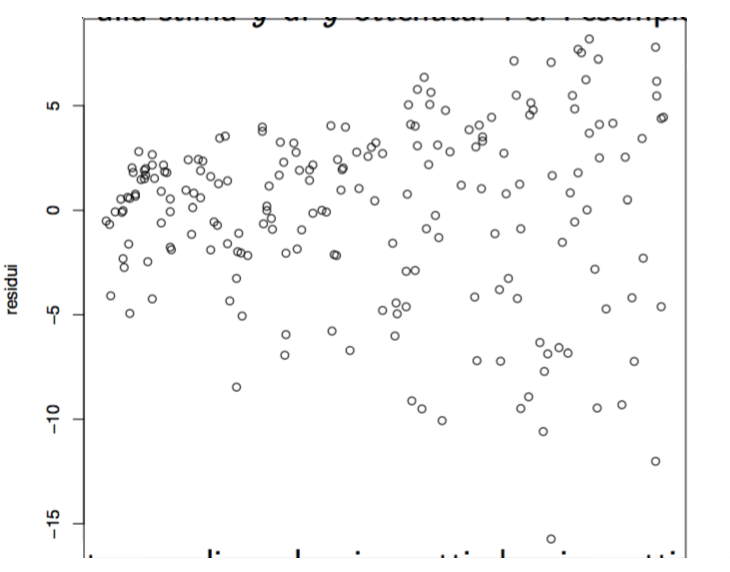
\includegraphics[width=.6\textwidth]{./notes/immagini/l6-fig12-1.png}
\caption{Residui rispetto $ \hat{y} $}
\end{figure}

Alternativamente, è possibile tracciare i residui rispetto alle \textit{x}. In questo modo è possibile osservare se la varianza è costante o se ci sono degli effetti sistematici che il modello non ha colto, oppure se il modello utilizzato non è adeguato.

\begin{figure}[htbp]
	\centering
	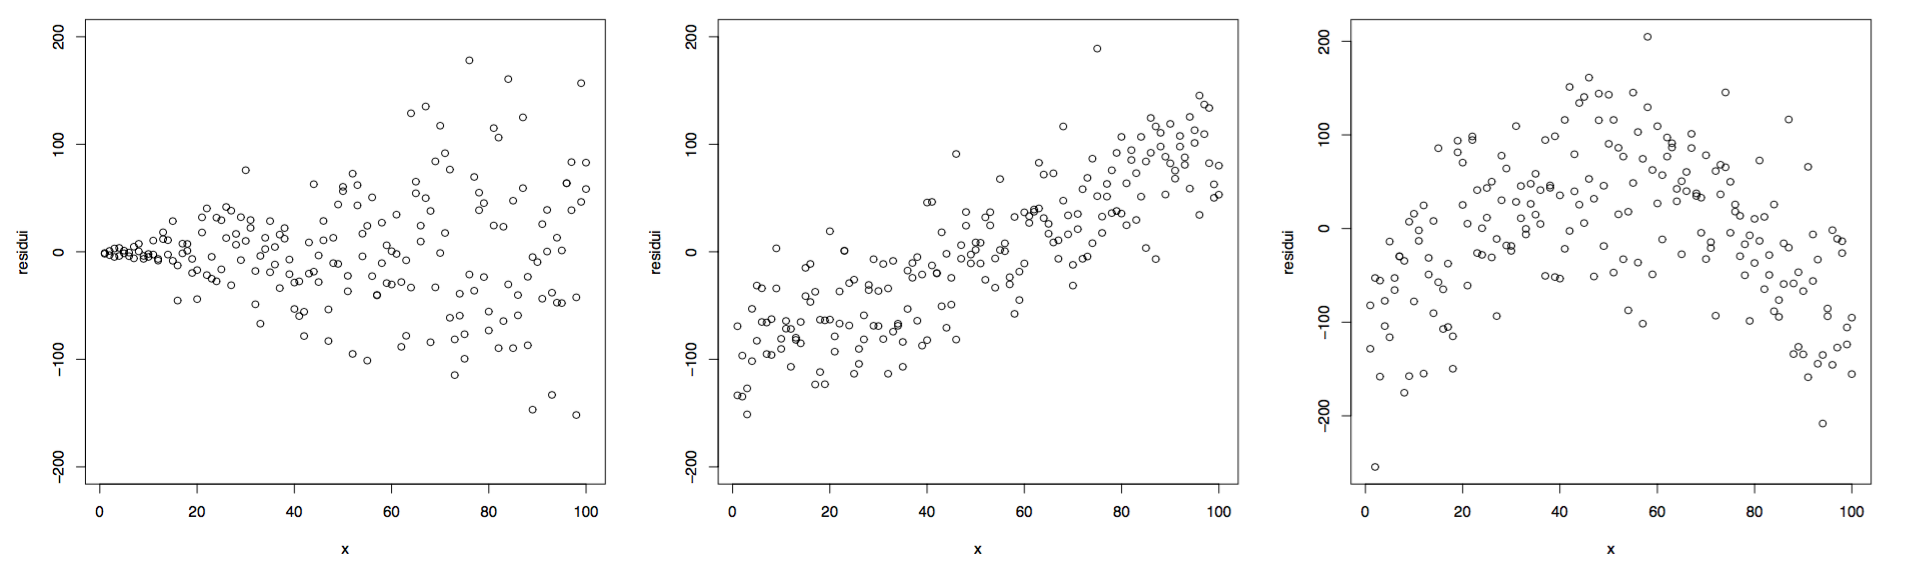
\includegraphics[width=\textwidth]{./notes/immagini/l6-fig13-1.png}
	\caption{Da sinistra verso destra: Varianza non costante, componente sistematica non considerata dal modello, modello inadeguato.}
\end{figure}


Dai grafici è possibile notare anche la presenza di valori anomali (\textbf{outliers}), osservazioni errate che non rispettano la distribuzione, che devono essere trattate in modo particolare per evitare che non influenzino in modo errato il modello.

Per verificare se la distribuzione è normale si può costruire un \textbf{qq-plot}.
Come prima cosa viene creata la distribuzione dei residui per i campioni osservati in modo che ogni punto sia caratterizzato dalla percentuale di punti minori o uguali rispetto alla totalità dei dati. Questa percentuale viene stimata utilizzando le varie frequenze.
Dopodiché è possibile confrontare i quantili della distribuzione ottenuta con quelli della normale standardizzata. Se per ciascuno punto i quantili sono circa uguali a quelli della normale, allora anche la distribuzione dei residui può essere considerata normale.

\begin{figure}[htbp]
	\centering
	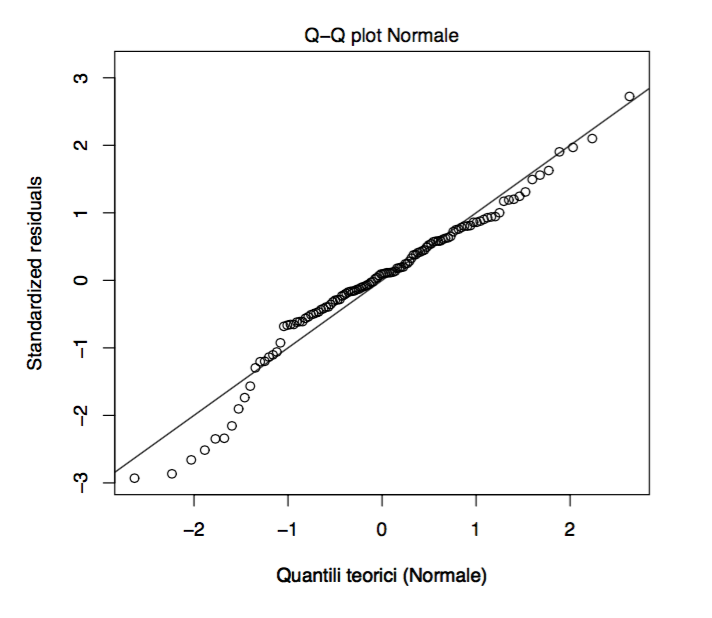
\includegraphics[width=.6\textwidth]{./notes/immagini/l6-fig14-1.png}
	\caption{QQ-Plot, tanto più i punti sono vicini alla bisettrice, tanto più la distribuzione può essere considerata normale.}
\end{figure}



